\documentclass[12pt,a4paper]{article}

% ─── Page Layout ───────────────────────────────────────────────────────────────
\usepackage[a4paper, margin=0.8in, headheight=14pt]{geometry}

% ─── Fonts (XeLaTeX) ───────────────────────────────────────────────────────────
\usepackage{fontspec}
\usepackage{unicode-math}
\setmainfont{TeX Gyre Pagella}
\setmonofont[Scale=0.88]{TeX Gyre Cursor}
\setmathfont{Latin Modern Math}

% ─── Packages ──────────────────────────────────────────────────────────────────
\usepackage{xcolor}
\usepackage{colortbl}
\usepackage{titlesec}
\usepackage{enumitem}
\usepackage{tabularx}
\usepackage{booktabs}
\usepackage{array}
\usepackage{amsmath}
\usepackage{tikz}
\usetikzlibrary{shapes.geometric, arrows.meta, positioning, calc, fit, decorations.pathreplacing, patterns}
\usepackage{tcolorbox}
\tcbuselibrary{skins, breakable}
\usepackage{hyperref}
\usepackage{fancyhdr}
\usepackage{graphicx}
\usepackage{microtype}
\hyphenpenalty=10000
\exhyphenpenalty=10000
\sloppy
\usepackage{caption}
\usepackage{setspace}
\usepackage{multirow}
\usepackage{tocloft}

% ─── Q&A helper ────────────────────────────────────────────────────────────────
\newcommand{\Q}[1]{\textbf{#1}\par\noindent\ignorespaces}

% ─── Colour Palette ────────────────────────────────────────────────────────────
\definecolor{myred}{RGB}{196,30,58}
\definecolor{mydark}{RGB}{30,30,50}
\definecolor{mygreen}{RGB}{14,120,80}
\definecolor{myteal}{RGB}{0,130,140}
\definecolor{myamber}{RGB}{180,100,0}
\definecolor{mypurple}{RGB}{100,30,160}
\definecolor{mygray}{RGB}{246,247,249}
\definecolor{mgframe}{RGB}{180,185,200}
\definecolor{watermark}{RGB}{145,150,170}
\definecolor{hdrred}{RGB}{250,232,235}
\definecolor{hdrgreen}{RGB}{220,244,233}
\definecolor{hdrteal}{RGB}{220,242,244}
\definecolor{hdramber}{RGB}{253,242,215}
\definecolor{hdrpurple}{RGB}{238,228,255}
\definecolor{hdrgray}{RGB}{238,240,245}
\definecolor{rowalt}{RGB}{250,251,253}

% ─── Section Formatting ────────────────────────────────────────────────────────
\titleformat{\section}
  {\large\bfseries\color{myred}}{\thesection.}{0.5em}{}
  [\vspace{1pt}{\color{myred}\rule{\linewidth}{0.8pt}}]
\titleformat{\subsection}
  {\normalsize\bfseries\color{myteal}}{\thesubsection}{0.5em}{}
\titlespacing*{\section}{0pt}{18pt}{7pt}
\titlespacing*{\subsection}{0pt}{11pt}{4pt}

% ─── Paragraph ─────────────────────────────────────────────────────────────────
\setlength{\parindent}{0pt}
\setlength{\parskip}{4pt}

% ─── TOC Styling ───────────────────────────────────────────────────────────────
\renewcommand{\cfttoctitlefont}{\large\bfseries\color{myred}}
\renewcommand{\cftaftertoctitle}{\par\noindent{\color{myred}\rule{\linewidth}{0.8pt}}}
\setlength{\cftbeforetoctitleskip}{0pt}
\setlength{\cftaftertoctitleskip}{6pt}
\renewcommand{\cftsecfont}{\normalsize\bfseries\color{mydark}}
\renewcommand{\cftsecpagefont}{\normalsize\bfseries\color{mydark}}
\renewcommand{\cftsecleader}{\cftdotfill{\cftdotsep}}
\setlength{\cftbeforesecskip}{7pt}
\renewcommand{\cftsubsecfont}{\small\color{mydark}}
\renewcommand{\cftsubsecpagefont}{\small\color{mydark}}
\setlength{\cftbeforesubsecskip}{3pt}
\setlength{\cftsubsecindent}{1.4em}

% ─── Table helpers ─────────────────────────────────────────────────────────────
\renewcommand{\arraystretch}{1.45}
\setlength{\tabcolsep}{6pt}
\arrayrulecolor{mydark}
\newcolumntype{B}[1]{>{\small\bfseries\raggedright\arraybackslash}m{#1}}
\newcolumntype{Y}{>{\small\raggedright\arraybackslash}X}
\renewcommand{\tabularxcolumn}[1]{m{#1}}

% ─── Header / Footer ───────────────────────────────────────────────────────────
\pagestyle{fancy}
\fancyhf{}
\fancyhead[L]{\small\color{myred}\textbf{EC401}\;\color{mydark}--- Analog Communication}
\fancyhead[R]{\small\color{myteal}\textbf{Module 4 Notes}}
\fancyfoot[C]{\small\color{mydark}\thepage}
\fancyfoot[R]{\small\color{watermark}\textit{\copyright\ Biraj}}
\renewcommand{\headrulewidth}{0.5pt}
\renewcommand{\footrulewidth}{0.3pt}

% ─── Hyperref ──────────────────────────────────────────────────────────────────
\hypersetup{
  colorlinks=true, linkcolor=myteal, urlcolor=myteal,
  pdfauthor={Biraj Sarkar (CGEC)},
  pdftitle={EC401 --- Module 4 Notes: Multiplexing, Stereo, Random Signals and Noise}
}

% ─── tcolorbox styles ──────────────────────────────────────────────────────────
\tcbset{
  tikzbox/.style={
    colback=mygray, colframe=mgframe, boxrule=0.6pt, arc=4pt,
    left=8pt, right=8pt, top=6pt, bottom=6pt,
    colbacktitle=mgframe, coltitle=mydark, fonttitle=\small\bfseries
  },
  defbox/.style={
    colback=hdrgreen, colframe=mygreen, boxrule=0.8pt, arc=4pt,
    left=9pt, right=9pt, top=6pt, bottom=6pt,
    colbacktitle=mygreen, coltitle=white, fonttitle=\small\bfseries
  },
  formulabox/.style={
    colback=hdrteal, colframe=myteal, boxrule=0.8pt, arc=4pt,
    left=9pt, right=9pt, top=7pt, bottom=7pt,
    colbacktitle=myteal, coltitle=white, fonttitle=\small\bfseries
  },
  examplebox/.style={
    colback=hdramber, colframe=myamber, boxrule=0.8pt, arc=4pt,
    left=9pt, right=9pt, top=6pt, bottom=6pt,
    colbacktitle=myamber, coltitle=white, fonttitle=\small\bfseries
  },
  masonbox/.style={
    colback=hdrpurple, colframe=mypurple, boxrule=0.8pt, arc=4pt,
    left=9pt, right=9pt, top=6pt, bottom=6pt,
    colbacktitle=mypurple, coltitle=white, fonttitle=\small\bfseries
  },
  exambox/.style={
    colback=hdrpurple, colframe=mypurple, boxrule=1pt, arc=5pt,
    left=10pt, right=10pt, top=8pt, bottom=8pt,
    colbacktitle=mypurple, coltitle=white, fonttitle=\bfseries,
    breakable, title after break={\textbf{Frequently Asked / Viva Questions (contd.)}}
  }
}
% Allow all boxes to break across pages — prevents footer overflow
\tcbset{breakable}
\tcbset{after={\color{black}}}

% ─── TikZ styles ───────────────────────────────────────────────────────────────
\tikzset{
  block/.style={rectangle, draw=myteal, fill=hdrteal,
    text width=2.4cm, align=center, minimum height=0.95cm,
    font=\small, rounded corners=3pt, line width=0.7pt},
  redblock/.style={rectangle, draw=myred, fill=hdrred,
    text width=2.4cm, align=center, minimum height=0.95cm,
    font=\small, rounded corners=3pt, line width=0.7pt},
  netnode/.style={rectangle, draw=myteal, fill=hdrteal,
    text width=1.5cm, align=center, minimum height=0.8cm,
    font=\small, rounded corners=3pt, line width=0.7pt},
  sumjunc/.style={circle, draw=myamber, fill=hdramber,
    minimum size=0.62cm, font=\small, line width=0.8pt},
  snode/.style={circle, draw=mypurple, fill=hdrpurple,
    minimum size=0.55cm, font=\footnotesize, line width=0.7pt},
  arrow/.style={-Stealth, thick, color=mydark},
  redarrow/.style={-Stealth, thick, color=myred},
  line/.style={thick, color=mydark}
  % ⚠ Do NOT define axis/.style here — conflicts with pgfplots/library keys.
  %   Use inline style instead: \draw[-Stealth, thin, color=mydark]
}

\begin{document}

% ─── Title Page ───────────────────────────────────────────────────────────────
\begin{center}
  {\LARGE\bfseries\color{myred} EC401 --- Analog Communication}\\[5pt]
  {\normalsize\color{mydark} Semester IV \quad$\bullet$\quad 3L:0T:0P \quad$\bullet$\quad 3 Credits}\\[3pt]
  {\normalsize\color{myteal}\textbf{Module 4 Exam Notes: Multiplexing, Stereo, Random Signals and Noise}}\\[3pt]
  {\small\color{mydark} CGEC \;$|$\; B.Tech ECE (2023--27) \;$|$\; \textit{Biraj Sarkar}}
\end{center}
\vspace{2pt}
\noindent{\color{myred}\rule{\linewidth}{1.5pt}}
\vspace{2pt}

\hypersetup{linkcolor=mydark}
\tableofcontents
\hypersetup{linkcolor=myteal}
\newpage

\section{Multiplexing and Stereo Transmission}
\subsection{Frequency Division Multiplexing}
\begin{tcolorbox}[defbox, title={FDM}]
Frequency division multiplexing translates each input to a distinct frequency band and adds the bands for simultaneous transmission. At the receiver, BPFs select the desired bands before demodulation. Guard bands allow realizable filter transitions and reduce adjacent-channel interference.
\end{tcolorbox}
If $N$ equal-width channels each occupy $B_{\rm ch}$ and adjacent channels have guard $g$, the span from the first occupied edge to the last is
\[
 B_{\rm span}=NB_{\rm ch}+(N-1)g.
\]
For four $3\,\mathrm{kHz}$ SSB channels with $1\,\mathrm{kHz}$ internal guards, this gives $4(3)+3(1)=15\,\mathrm{kHz}$. External allocation margins, if specified, must be added separately.

\begin{tcolorbox}[tikzbox, unbreakable, title={FDM Channels and Guard Bands}]
\centering
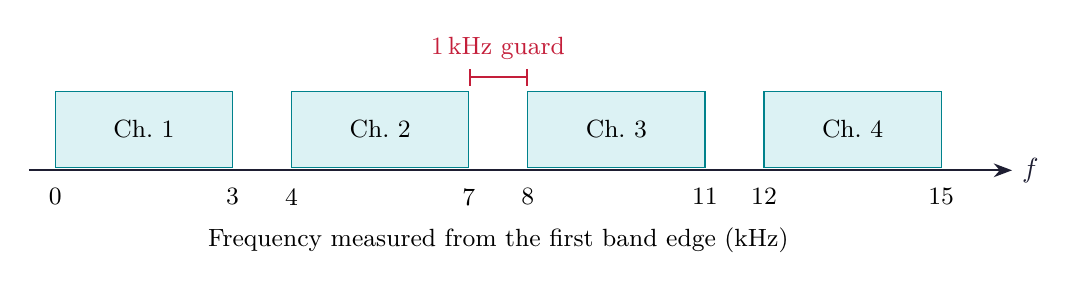
\begin{tikzpicture}[x=0.75cm]
  \draw[arrow] (-0.45,0)--(16.2,0) node[right] {$f$};
  \foreach \a/\b/\ch in {0/3/1,4/7/2,8/11/3,12/15/4}{
    \filldraw[fill=hdrteal,draw=myteal] (\a,0.04) rectangle (\b,1);
    \node at ({(\a+\b)/2},0.52) {\small Ch.\ \ch};
    \node[below=3pt] at (\a,0) {\small \a};
    \node[below=3pt] at (\b,0) {\small \b};
  }
  \draw[|-|,myred,thick] (7,1.18)--(8,1.18);
  \node[above=3pt,myred] at (7.5,1.18) {\small $1\,\mathrm{kHz}$ guard};
  \node[below] at (7.5,-0.6) {\small Frequency measured from the first band edge (kHz)};
\end{tikzpicture}\par
\end{tcolorbox}

\subsection{Time Division Multiplexing}
\begin{tcolorbox}[defbox, title={Synchronous TDM}]
Time division multiplexing assigns successive time slots to different inputs. In analog PAM-TDM, a clocked commutator samples each band-limited input once per frame. A synchronized receiver routes slots back to their channels and reconstruction LPFs recover the messages.
\end{tcolorbox}
For equal channel bandwidth $W$, each frame must recur at $f_s\ge 2W$ in the ideal sampling model. With $N$ equal slots and $n_{\rm ov}$ additional synchronization slots per frame,
\[
 R_{\rm slot}=(N+n_{\rm ov})f_s,\qquad
 T_{\rm slot}=\frac{1}{R_{\rm slot}}.
\]
Three channels limited to $3\,\mathrm{kHz}$ can be sampled at $8\,\mathrm{kHz}$ each. With one framing slot, the aggregate is $32\,\mathrm{kslot/s}$ and each slot is $31.25\,\mu\mathrm{s}$. Pulse shape, guard time and filtering determine required channel bandwidth. The slot rate alone does not specify it.

\begin{tcolorbox}[tikzbox, unbreakable, title={Two Frames of Three-Channel TDM}]
\centering
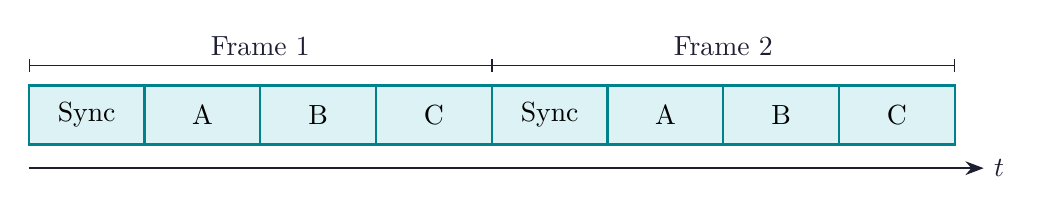
\begin{tikzpicture}[x=1.47cm]
  \foreach \x/\lab in {0/Sync,1/A,2/B,3/C,4/Sync,5/A,6/B,7/C}{
    \draw[thick,draw=myteal,fill=hdrteal] (\x,0) rectangle ++(1,0.75);
    \node at (\x+0.5,0.38) {\lab};
  }
  \draw[|-|,mydark] (0,1)--(4,1) node[midway,above] {Frame 1};
  \draw[|-|,mydark] (4,1)--(8,1) node[midway,above] {Frame 2};
  \draw[arrow] (0,-0.3)--(8.25,-0.3) node[right] {$t$};
\end{tikzpicture}\par
\end{tcolorbox}

FDM requires separate frequency slots and filter selectivity. TDM needs sample timing and frame synchronization. FDM is used in broadcast channel allocation and multicarrier links. TDM is used in shared sampled-data and telephone links.

\subsection{FM Stereo}
Form the sum $S=L+R$ and difference $D=L-R$. A pilot-tone stereo multiplex carries $S$ in the $0$--$15\,\mathrm{kHz}$ band, a $19\,\mathrm{kHz}$ pilot, and DSB-SC $D$ around $38\,\mathrm{kHz}$, occupying $23$--$53\,\mathrm{kHz}$. This composite controls the FM transmitter. A mono receiver recovers the low-pass sum. A stereo receiver locks to the pilot, regenerates the $38\,\mathrm{kHz}$ subcarrier, coherently detects $D$, and reconstructs
\[
 L=\frac{S+D}{2},\qquad R=\frac{S-D}{2}.
\]
Pilot recovery and matched audio paths maintain stereo separation. Without a usable pilot the receiver can fall back to mono.

\begin{tcolorbox}[tikzbox, unbreakable, title={FM Stereo Encoder and Decoder}]
\centering
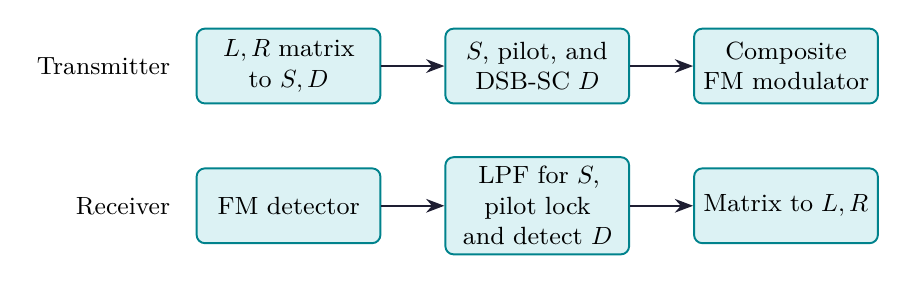
\begin{tikzpicture}[node distance=8mm,sblock/.style={block,text width=2.1cm}]
  \node[sblock] (m) {$L,R$ matrix to $S,D$};
  \node[sblock,right=of m] (c) {$S$, pilot, and DSB-SC $D$};
  \node[sblock,right=of c] (t) {Composite FM modulator};
  \draw[arrow] (m)--(c); \draw[arrow] (c)--(t);
  \node[sblock,below=8mm of m] (r) {FM detector};
  \node[sblock,right=of r] (d) {LPF for $S$, pilot lock and detect $D$};
  \node[sblock,right=of d] (o) {Matrix to $L,R$};
  \draw[arrow] (r)--(d); \draw[arrow] (d)--(o);
  \node[anchor=east] at ([xshift=-2mm]m.west) {\small Transmitter};
  \node[anchor=east] at ([xshift=-2mm]r.west) {\small Receiver};
\end{tikzpicture}\par
\end{tcolorbox}

\begin{tcolorbox}[examplebox, title={Trace and Recover the FM Stereo Channels}]
A left-only $8\,\mathrm{kHz}$ tone $L(t)$ enters the encoder, with $R(t)=0$. The sum and difference signals both equal $L(t)$.
\begin{itemize}[leftmargin=*, itemsep=3pt]
 \item The sum occupies baseband at $8\,\mathrm{kHz}$. A mono receiver passes it directly.
 \item The difference modulates the suppressed $38\,\mathrm{kHz}$ subcarrier. Its two lines lie at $30$ and $46\,\mathrm{kHz}$. A pilot at $19\,\mathrm{kHz}$ supplies the receiver's phase reference.
 \item After product detection and low-pass filtering, the decoder obtains $S=D=L(t)$. The matrix therefore gives $(S+D)/2=L(t)$ and $(S-D)/2=0$.
\end{itemize}
If the regenerated subcarrier has phase error $\theta$, the recovered difference is scaled by $\cos\theta$ in the ideal product detector. The unwanted right-channel output is then $L(t)(1-\cos\theta)/2$, showing how phase mismatch reduces stereo separation.
\end{tcolorbox}

\subsection{Compatible AM Stereo}
In a representative C-QUAM system the normalized mono sum controls the AM envelope, while the difference controls a quadrature phase component. With $a(t)=1+k_s S(t)>0$, $b(t)=k_dD(t)$ and $\phi=\tan^{-1}(b/a)$,
\[
\begin{aligned}
 q(t)&=a\cos\omega_ct-b\sin\omega_ct
      =\sqrt{a^2+b^2}\cos(\omega_ct+\phi),\\
 s(t)&=A_cq(t)\cos\phi
      =A_c a(t)\cos(\omega_ct+\phi).
\end{aligned}
\]
An ordinary envelope detector therefore recovers the mono sum after DC removal. A compatible stereo receiver recovers that sum, uses coherent quadrature detection with cosine correction to recover the difference, and applies the $S,D$ matrix. A stereo identification pilot can signal when to decode the difference. The diagram shows the principle rather than hardware for a particular receiver.

\begin{tcolorbox}[tikzbox, unbreakable, title={Compatible AM Stereo Signal Paths}]
\centering
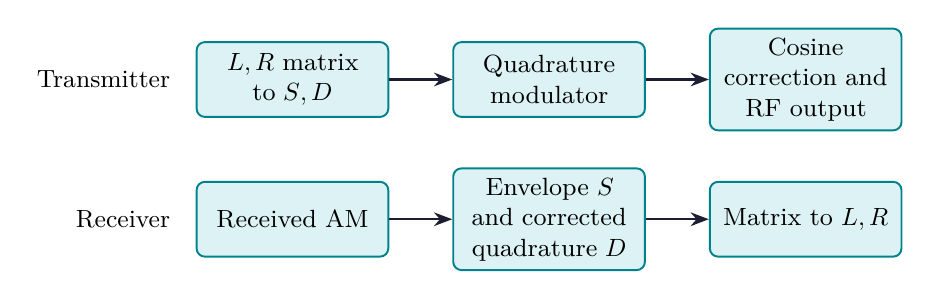
\begin{tikzpicture}[node distance=8mm,sblock/.style={block,text width=2.2cm}]
  \node[sblock] (m) {$L,R$ matrix to $S,D$};
  \node[sblock,right=of m] (q) {Quadrature modulator};
  \node[sblock,right=of q] (tx) {Cosine correction and RF output};
  \draw[arrow] (m)--(q); \draw[arrow] (q)--(tx);
  \node[sblock,below=8mm of m] (rf) {Received AM};
  \node[sblock,right=of rf] (de) {Envelope $S$ and corrected quadrature $D$};
  \node[sblock,right=of de] (lr) {Matrix to $L,R$};
  \draw[arrow] (rf)--(de); \draw[arrow] (de)--(lr);
  \node[anchor=east] at ([xshift=-2mm]m.west) {\small Transmitter};
  \node[anchor=east] at ([xshift=-2mm]rf.west) {\small Receiver};
\end{tikzpicture}\par
\end{tcolorbox}
\par\smallskip
{\small See these stereo and multiplex references.

\href{https://patents.google.com/patent/US4170716A/en}{Motorola compatible AM stereo receiver}
and \href{https://www.itu.int/rec/R-REC-BS.450/en}{ITU-R BS.450}.\par}

\section{Random Signals and Noise in Communication}
\subsection{Noise Sources and Random Processes}
A random process $X(t)$ is a family of random variables indexed by time. Each realization is a waveform. A wide-sense stationary process has constant mean and autocorrelation depending only on lag, $R_X(\tau)=E[X(t)X(t+\tau)]$ for real $X$. Its power spectral density (PSD) is the Fourier transform of $R_X(\tau)$. An LTI filter changes an input PSD $S_X$ to $|H(f)|^2 S_X(f)$.

\par\vspace{6pt}
\begingroup
\setlength{\extrarowheight}{3pt}
\noindent\begin{tabularx}{\linewidth}{|B{3.3cm}|Y|Y|}
\hline
\multicolumn{1}{|c|}{\textbf{Class}} & \multicolumn{1}{c|}{\textbf{Origins}} & \multicolumn{1}{c|}{\textbf{Engineering response}}\\
\hline
External & Atmospheric lightning, solar and galactic radiation, industrial and switching interference. & Antenna placement, shielding, grounding and RF selectivity.\\
\hline
Internal & Thermal agitation, shot noise from discrete charge flow and low-frequency flicker noise. & Low-noise front end, suitable bias and limited noise bandwidth.\\
\hline
\end{tabularx}\par
\endgroup

\subsection{White Noise, Thermal Noise and Noise Temperature}
\begin{tcolorbox}[formulabox, title={Noise Power and SNR}]
White noise has constant PSD across the band of interest. With a two-sided PSD $N_0/2$, ideal white noise passed by an LPF of cutoff $W$ has power $N_0 W$. Ideal whiteness over infinite bandwidth is a model. AWGN means additive, white and Gaussian noise. Gaussian describes the amplitude distribution, whereas whiteness describes the spectrum.

For a resistor at temperature $T$, the classical one-sided open-circuit voltage PSD is $4kTR$ in $\mathrm{V^2/Hz}$. A matched load sees half the open-circuit voltage. Across bandwidth $B$,
\[
\begin{aligned}
 \overline{v_{\rm load}^2}&=\frac{4kTRB}{4}=kTRB,\\
 P_N&=\frac{\overline{v_{\rm load}^2}}{R}=kTB\quad(\mathrm W),\\
 \mathrm{SNR}&=\frac{P_s}{P_N},\quad
 \mathrm{SNR}_{\rm dB}=10\log_{10}(P_s/P_N).
\end{aligned}
\]
Here $k=1.380649\times10^{-23}\,\mathrm{J/K}$. Use equivalent noise bandwidth for a nonrectangular filter.
\end{tcolorbox}

Equivalent input noise temperature $T_e$ expresses receiver-added noise as an input source $kT_eB$. For source noise temperature $T_A$, input-referred system noise is $k(T_A+T_e)B$. Noise factor $F$ is input SNR divided by output SNR at the reference input temperature $T_0=290\,\mathrm K$:
\[
 F=1+\frac{T_e}{T_0},\qquad NF=10\log_{10}F.
\]
Cascaded input-referred temperatures are $T_{e1}+T_{e2}/G_1+\cdots$, because the equivalent noise of each later stage is divided by preceding linear power gain.

\begin{tcolorbox}[examplebox, title={Noise Temperature and Input-Referred SNR}]
A receiver has $F=2$, an antenna has $T_A=150\,\mathrm K$, and $B=10\,\mathrm{kHz}$. Received signal power is $10^{-13}\,\mathrm W$.
\[
\begin{aligned}
 T_e&=(2-1)(290)=290\,\mathrm K,\\
 T_{\rm sys}&=150+290=440\,\mathrm K,\\
 P_N&=(1.380649\times10^{-23})(440)(10^4)\,\mathrm W\\
    &\approx6.07\times10^{-17}\,\mathrm W,\\
 \mathrm{SNR}_{\rm dB}&=10\log_{10}\!\left(\frac{10^{-13}}{6.07\times10^{-17}}\right)
             \approx32.2\,\mathrm{dB}.
\end{aligned}
\]
\end{tcolorbox}

\begin{tcolorbox}[examplebox, title={Calculate a Two-Stage Receiver Noise Temperature}]
The first amplifier has gain $G_1=10$ and input-referred noise temperature $T_{e1}=70\,\mathrm K$. The converter that follows has $T_{e2}=400\,\mathrm K$.
\[
\begin{aligned}
 T_e &= T_{e1}+\frac{T_{e2}}{G_1}
      =70+\frac{400}{10}=110\,\mathrm K,\\
 F&=1+\frac{T_e}{290}=1.379,\qquad
 NF=10\log_{10}F\approx1.40\,\mathrm{dB}.
\end{aligned}
\]
With an antenna at $120\,\mathrm K$, the total input-referred system temperature is $230\,\mathrm K$. For a $200\,\mathrm{kHz}$ noise bandwidth the available noise is
\[
 P_N=k(230)(200\,000)\approx6.35\times10^{-16}\,\mathrm W.
\]
The later converter contributes only $40\,\mathrm K$ referred to the input because the preceding amplifier has gain ten. In cascade formulas use linear gain and noise factor, then convert to decibels if required.
\end{tcolorbox}

\section{Noise Performance of Analog Modulation}
\subsection{Reference SNR and Detection Assumptions}
Let $W$ be the baseband bandwidth and $N_0/2$ the two-sided RF noise PSD. Express powers at a normalized $1\,\Omega$ load. Let $P_R$ be total received RF signal power, including any transmitted carrier, and $P_U$ its information-bearing RF power. Use the same baseband reference for every scheme:
\[
 \gamma_{\rm ref}=\frac{P_R}{N_0W},\qquad
 \mathcal F=\frac{\mathrm{SNR}_{\rm out}}{\gamma_{\rm ref}}.
\]
This figure of merit $\mathcal F$ uses a common reference rather than actual RF-filter input SNR. A rectangular RF filter of positive-frequency bandwidth $B_{\rm RF}$ passes noise power $N_0B_{\rm RF}$, giving actual RF input SNR $P_R/(N_0B_{\rm RF})$. If a question uses that denominator, multiply $\mathcal F$ by $B_{\rm RF}/W$.

\subsection{DSB-TC, DSB-SC, SSB-TC and SSB-SC}
Ideal coherent detection uses $2\cos(2\pi f_ct)$ and a baseband LPF. For DSB, the shifted positive and negative RF noise bands both contribute across $|f|\le W$. Thus $S_{n,\rm out}=N_0$, giving $2N_0W$. The useful waveform $u(t)\cos\omega_ct$ has $P_U=E[u^2]/2$. Its baseband useful power is $E[u^2]=2P_U$, so
\[
 \mathrm{SNR}_{\rm out,DSB}=\frac{2P_U}{2N_0W}=\frac{P_U}{N_0W}.
\]
For DSB-TC the carrier becomes DC and is removed. At high carrier-to-noise ratio with a positive envelope, the envelope detector also yields the in-phase noise to first order. For the single tone, $P_U/P_R=\mu^2/(2+\mu^2)$. DSB-SC uses all of $P_R$ for the useful sidebands.

For SSB, $s_U(t)=u(t)\cos\omega_ct-\widehat u(t)\sin\omega_ct$. With zero-mean $u$, the Hilbert transform has the same power, so
\[
 P_U=\tfrac12[E(u^2)+E(\widehat u^2)]=E(u^2).
\]
Only one translated noise contribution remains at each nonzero baseband frequency, giving $S_{n,\rm out}=N_0/2$ and $N_0W$ in-band noise. Coherent SSB detection therefore also gives $P_U/(N_0W)$. SSB-SC has $P_R=P_U$. SSB-TC has $P_R=P_U+P_c$. The carrier becomes removable DC. A strong-carrier envelope detector can approximate coherent output to first order, with quadrature distortion as the carrier becomes less dominant.

\begin{tcolorbox}[formulabox, title={Track the RF Noise through the Product Detector}]
The oscillator $2\cos(2\pi f_ct)$ translates RF noise to baseband through two unit-amplitude frequency shifts. For filtered, wide-sense stationary noise with RF PSD $S_{n,\rm RF}$, the time-averaged baseband PSD is
\[
 S_{n,\rm out}(f)=S_{n,\rm RF}(f-f_c)+S_{n,\rm RF}(f+f_c),
 \qquad |f|\le W .
\]
The two separated RF contributions have uncorrelated spectral increments. A DSB RF filter passes both terms at each in-band $f$, yielding $N_0$. An SSB RF filter passes one, yielding $N_0/2$. The carrier line in a transmitted-carrier scheme shifts to DC and is removed when calculating useful audio power.
\end{tcolorbox}

\begin{tcolorbox}[examplebox, title={Keep Reference SNR and RF Input SNR Separate}]
For DSB-TC, let $P_R=2\,\mathrm{mW}$, $W=4\,\mathrm{kHz}$, $N_0=5\times10^{-10}\,\mathrm{W/Hz}$ and tone index $\mu=0.5$. The RF filter has $B_{\rm RF}=2W$.
\[
\begin{aligned}
 \gamma_{\rm ref} &=\frac{2\times10^{-3}}{(5\times10^{-10})(4000)}=1000,\\
 \gamma_{\rm RF,in}&=\frac{2\times10^{-3}}{(5\times10^{-10})(8000)}=500,\\
 \eta &= \frac{\mu^2}{2+\mu^2}=\frac19,\\
 \gamma_{\rm out}&=\eta\gamma_{\rm ref}=\frac{1000}{9}\approx111.1 .
\end{aligned}
\]
The figure of merit under the common-reference convention is $1/9$. Under the actual RF input convention it is $111.1/500\approx2/9$. The receiver and its output SNR are the same in both calculations.
\end{tcolorbox}

\subsection{FM Discriminator Noise Above Threshold}
A limiter removes amplitude variations. Let the received FM amplitude be $A$, so that $P_R=A^2/2$. For high predetection carrier-to-noise ratio, received quadrature noise $n_Q(t)$ gives a small phase error $n_Q/A$. Ideal broad predetection filtering gives quadrature noise PSD approximately $N_0$ over the output band. A unity-frequency-gain discriminator followed by scaling by $1/k_f$ gives the output $m(t)$ plus
\[
\begin{aligned}
 n_o(t)&\approx \frac{1}{2\pi A k_f}\frac{d n_Q(t)}{dt},\\
 S_{n_o}(f)&\approx \frac{N_0 f^2}{A^2 k_f^2},\qquad |f|\le W,\\
 P_{n_o}&=\int_{-W}^{W}S_{n_o}(f)\,df
          =\frac{2N_0 W^3}{3A^2k_f^2},\\
 \mathrm{SNR}_{\rm out,FM}
      &\approx\frac{3P_Rk_f^2P_m}{N_0W^3},
      \qquad P_m=E[m^2(t)].
\end{aligned}
\]
For a full-band tone with $f_m=W$, $P_m=A_m^2/2$ and $\Delta f=k_f A_m$. Hence $\mathcal F_{\rm FM}\approx\tfrac32(\Delta f/W)^2$. The noise voltage density grows with frequency, and noise PSD grows as $f^2$. Pre-emphasis boosts high audio frequencies before transmission and complementary de-emphasis reduces their noise after detection. Below threshold, large phase errors produce clicks and the small-noise formula no longer applies.

\begin{tcolorbox}[tikzbox, unbreakable, title={FM Discriminator Output Noise PSD}]
\centering
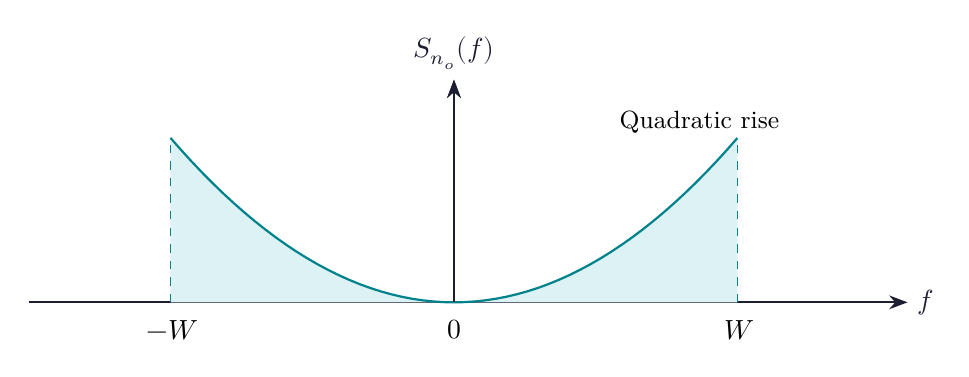
\begin{tikzpicture}[x=1.8cm,y=1.45cm]
  \draw[arrow] (-3,0)--(3.2,0) node[right] {$f$};
  \draw[arrow] (0,0)--(0,1.95) node[above] {$S_{n_o}(f)$};
  \fill[hdrteal,domain=-2:2,samples=55] (-2,0)--plot (\x,{0.36*\x*\x})--(2,0)--cycle;
  \draw[myteal,thick,domain=-2:2,samples=55] plot (\x,{0.36*\x*\x});
  \draw[dashed,myteal] (-2,0)--(-2,1.44) (2,0)--(2,1.44);
  \draw[arrow] (0,0)--(0,1.95);
  \node[below=3pt] at (-2,0) {$-W$};
  \node[below=3pt] at (0,0) {$0$};
  \node[below=3pt] at (2,0) {$W$};
  \node[right] at (1.1,1.58) {\small Quadratic rise};
\end{tikzpicture}\par
\end{tcolorbox}

\begin{tcolorbox}[examplebox, title={Compare Five Schemes at Equal Total Received Power}]
Let $\gamma_{\rm ref}=100$ ($20\,\mathrm{dB}$). Use conventional AM with $\mu=0.8$, SSB-TC with $P_c=3P_U$, and full-band tone FM with $\Delta f/W=4$ above threshold. Under the respective detection assumptions:
\[
\begin{aligned}
 \gamma_{\rm DSB-TC}&=100\frac{0.8^2}{2+0.8^2}
          \approx24.24\quad(13.85\,\mathrm{dB}),\\
 \gamma_{\rm DSB-SC}&=100\quad(20\,\mathrm{dB}),\\
 \gamma_{\rm SSB-TC}&=100\frac{1}{1+3}
          =25\quad(13.98\,\mathrm{dB}),\\
 \gamma_{\rm SSB-SC}&=100\quad(20\,\mathrm{dB}),\\
 \gamma_{\rm FM}&\approx100\left(\frac32\right)4^2
          =2400\quad(33.80\,\mathrm{dB}).
\end{aligned}
\]
The FM improvement uses a larger RF bandwidth. Carrier suppression avoids using part of the total power in a non-message component.
\end{tcolorbox}
\par\smallskip
{\small Further reading on figure of merit and detector noise.

\href{https://archive.nptel.ac.in/content/storage2/courses/117106090/Pdfs/1_10.pdf}{IIT Madras Principles of Communication noise analysis}.\par}

\section{Probability and Signal Distributions}
\subsection{Joint Probability, Conditioning and Independence}
For $P(B)>0$, the joint probability of $A$ and $B$ and its conditional form obey
\[
 P(A\cap B)=P(A\mid B)P(B),\qquad
 P(A\mid B)=\frac{P(A\cap B)}{P(B)}.
\]
Independence means $P(A\cap B)=P(A)P(B)$. For two random variables it means the joint CDF factors. Where joint densities exist, the joint density equals the product of marginals almost everywhere. Summing a joint PMF or integrating a joint PDF over one variable gives the other marginal.

\begin{tcolorbox}[examplebox, title={Infer a Transmitted Bit from the Detected Bit}]
Let $P(T=1)=0.3$, $P(R=1\mid T=1)=0.9$, and $P(R=1\mid T=0)=0.1$.
\[
\begin{aligned}
 P(T=1,R=1)&=0.9(0.3)=0.27,\\
 P(R=1)&=0.9(0.3)+0.1(0.7)=0.34,\\
 P(T=1\mid R=1)&=\frac{0.27}{0.34}\approx0.794.
\end{aligned}
\]
Since $P(T=1\mid R=1)\ne P(T=1)$, the detected and transmitted bits are statistically dependent.
\end{tcolorbox}

\subsection{Discrete and Continuous Random Variables}
A discrete random variable has a probability mass function (PMF) $p_X(x)=P(X=x)$. For a continuous variable with density $f_X$, probabilities are integrals of nonnegative density, with total integral one. A density has units inverse to the variable units. The cumulative distribution function (CDF) is always $F_X(x)=P(X\le x)$:
\[
 \begin{aligned}
 F_X(x)&=\sum_{x_i\le x}p_X(x_i) && \text{(discrete)},\\
 F_X(x)&=\int_{-\infty}^{x}f_X(u)\,du && \text{(continuous)},\\
 P(a<X\le b)&=F_X(b)-F_X(a).
 \end{aligned}
\]
For a differentiable continuous CDF, $f_X=F_X'$. A discrete CDF jumps at each point of positive mass. A continuous variable with a PDF has $P(X=x)=0$ at a single point.

\subsection{Gaussian, Rayleigh and Rician Densities}
\begin{tcolorbox}[formulabox, title={Three Communication Distributions}]
\textbf{Gaussian.} For mean $\mu$ and variance $\sigma^2$, the PDF is
\[
 f_X(x)=\frac{1}{\sigma\sqrt{2\pi}}\exp\!\left[-\frac{(x-\mu)^2}{2\sigma^2}\right],
 \qquad -\infty<x<\infty.
\]
The CDF is $F_X(x)=\Phi((x-\mu)/\sigma)$, with $\Phi$ the standard normal CDF. Gaussian noise is used for receiver thermal noise.

\textbf{Rayleigh.} With independent zero-mean Gaussian quadratures of variance $\sigma^2$, their envelope $R=\sqrt{I^2+Q^2}$ is Rayleigh. Transforming to polar coordinates multiplies the joint density by the Jacobian $r$. Integrating the angle over $2\pi$ gives
\[
 f_R(r)=\frac{r}{\sigma^2}e^{-r^2/(2\sigma^2)},\qquad
 F_R(r)=1-e^{-r^2/(2\sigma^2)},\qquad r\ge0.
\]
Both are zero for $r<0$. This envelope model is used for diffuse multipath without a dominant component.

\textbf{Rician.} With a deterministic phasor of magnitude $a$ and diffuse Gaussian quadratures of variance $\sigma^2$ each,
\[
 f_R(r)=\frac{r}{\sigma^2}
        e^{-(r^2+a^2)/(2\sigma^2)} I_0\!\left(\frac{ra}{\sigma^2}\right),
        \qquad r\ge0.
\]
The PDF is zero for negative $r$. Here $I_0$ is the modified Bessel function of order zero, arising from angular integration of the shifted Gaussian density. The CDF is $\int_0^r f_R(u)\,du$ for $r\ge0$. The ratio of deterministic to diffuse power is $K=a^2/(2\sigma^2)$. At $a=0$, $I_0(0)=1$ and the density becomes Rayleigh.
\end{tcolorbox}

\subsection{Derive the Envelope Distributions from Gaussian Quadratures}
For independent quadrature voltages $I,Q\sim\mathcal N(0,\sigma^2)$, write $i=r\cos\theta$ and $q=r\sin\theta$. The area element changes from $di\,dq$ to $r\,dr\,d\theta$. Therefore the joint density of radius and angle and its marginal are
\[
\begin{aligned}
 f_{R,\Theta}(r,\theta)
   &=\frac{r}{2\pi\sigma^2}\exp[-r^2/(2\sigma^2)],\\
 f_R(r)&=\int_0^{2\pi} f_{R,\Theta}(r,\theta)\,d\theta
        =\frac{r}{\sigma^2}e^{-r^2/(2\sigma^2)},\\
 F_R(r)&=\int_0^r\frac{u}{\sigma^2}e^{-u^2/(2\sigma^2)}\,du
        =\left[-e^{-u^2/(2\sigma^2)}\right]_0^r .
\end{aligned}
\]
Now choose the in-phase axis along a deterministic phasor so $I\sim\mathcal N(a,\sigma^2)$ and $Q\sim\mathcal N(0,\sigma^2)$ remain independent. The shifted quadratic becomes
\[
 (i-a)^2+q^2=r^2+a^2-2ra\cos\theta.
\]
After the same Jacobian and angular integration,
\[
\begin{aligned}
 f_R(r)&=\frac r{\sigma^2}e^{-(r^2+a^2)/(2\sigma^2)}
          \left[\frac{1}{2\pi}\int_0^{2\pi}
                 e^{(ra/\sigma^2)\cos\theta}\,d\theta\right],\\
       &=\frac r{\sigma^2}e^{-(r^2+a^2)/(2\sigma^2)}
                       I_0(ra/\sigma^2),\qquad r\ge0.
\end{aligned}
\]
This is the Rician density. Setting $a=0$ makes the bracket one and gives the Rayleigh density. The Gaussian model describes the signed quadrature voltages. Their nonnegative magnitude follows the envelope model.

\begin{tcolorbox}[tikzbox, unbreakable, title={Gaussian, Rayleigh and Rician Density Shapes}]
\centering
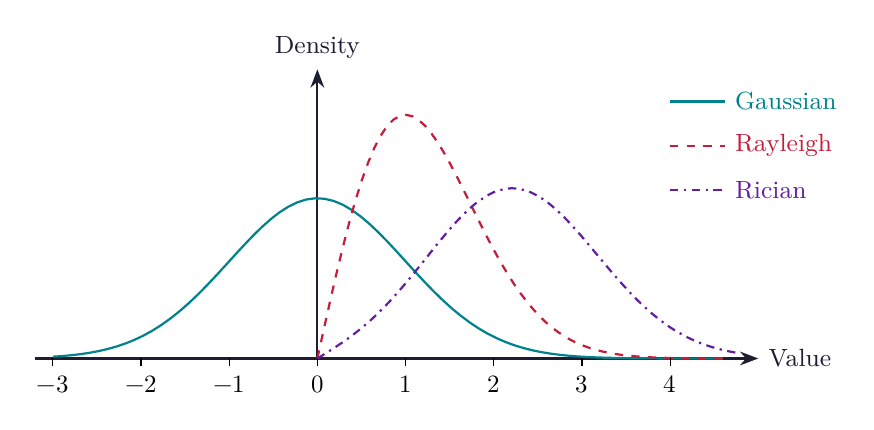
\begin{tikzpicture}[x=1.12cm,y=5.1cm,every node/.style={font=\small}]
  \draw[arrow] (-3.2,0)--(5.0,0) node[right] {Value};
  \draw[arrow] (0,0)--(0,0.72) node[above] {Density};
  \draw[myteal,thick,domain=-3:4.6,samples=75] plot (\x,{0.398942*exp(-\x*\x/2)});
  \draw[myred,thick,dashed,domain=0:4.6,samples=65] plot (\x,{\x*exp(-\x*\x/2)});
  \draw[mypurple,thick,dashdotted] plot[smooth] coordinates {
    (0.0,0.0000) (0.2,0.0276) (0.4,0.0583) (0.6,0.0945) (0.8,0.1376) (1.0,0.1871) (1.2,0.2410) (1.4,0.2956) (1.6,0.3460)
    (1.8,0.3870) (2.0,0.4140) (2.2,0.4239) (2.4,0.4156) (2.6,0.3904) (2.8,0.3514) (3.0,0.3032) (3.2,0.2509)
    (3.4,0.1992) (3.6,0.1516) (3.8,0.1108) (4.0,0.0776) (4.2,0.0522) (4.4,0.0337) (4.6,0.0209) (4.8,0.0124)
  };
  \foreach \x in {-3,-2,-1,0,1,2,3,4}{
    \draw (\x,0)--(\x,-0.018) node[below] {$\x$};
  }
  \draw[myteal,thick] (4,0.64)--(4.62,0.64) node[right] {Gaussian};
  \draw[myred,thick,dashed] (4,0.53)--(4.62,0.53) node[right] {Rayleigh};
  \draw[mypurple,thick,dashdotted] (4,0.42)--(4.62,0.42) node[right] {Rician};
\end{tikzpicture}\par
\small Here $\sigma=1$ in all three models, $\mu=0$ for the Gaussian, and $a=2$ for the Rician. The Gaussian can take negative values. The envelope distributions start at zero.
\end{tcolorbox}

\begin{tcolorbox}[examplebox, title={Rayleigh Envelope Outage}]
For Rayleigh quadrature scale $\sigma=1\,\mathrm V$ and a receiver threshold $r_0=0.5\,\mathrm V$,
\[
 P(R<r_0)=F_R(r_0)=1-e^{-(0.5)^2/2}\approx0.1175.
\]
Roughly $11.75\%$ of envelope samples fall below the threshold under this model.
\end{tcolorbox}

\begin{tcolorbox}[masonbox, title={Exam Checks}]
Use actual RF noise bandwidth for RF-filter noise power and the stated reference bandwidth for figure of merit. Convert power ratios with $10\log_{10}$. State the limiting assumptions for envelope or FM noise analysis. For amplitude statistics, distinguish the Gaussian quadratures from their nonnegative envelope.
\end{tcolorbox}


\newpage
\begin{center}
  {\large\bfseries\color{myred} Quick Revision --- Module 4}\\[3pt]
  {\small\color{mydark} Multiplexing, Stereo, Random Signals and Noise $|$ EC401}
\end{center}
\noindent{\color{myred}\rule{\linewidth}{1.2pt}}
\par\vspace{4pt}

\begin{tcolorbox}[formulabox, title={Key Formulas at a Glance}]
\renewcommand{\arraystretch}{1.35}
\noindent\begin{tabularx}{\linewidth}{B{4.4cm} Y}
FDM and TDM & $B_{\rm span}=NB_{\rm ch}+(N-1)g$ \newline $R_{\rm slot}=(N+n_{\rm ov})f_s$ \\[4pt]
Stereo matrix & $S=L+R,\ D=L-R$ \newline $L=(S+D)/2,\ R=(S-D)/2$ \\[4pt]
Thermal noise & $P_N=kTB$ \quad $T_e=(F-1)T_0$ \\[4pt]
AM and SSB output SNR & $P_U/(N_0W)$ under the stated detection assumptions \\[4pt]
FM above threshold & $\mathrm{SNR}_{\rm out}\approx3P_R k_f^2P_m/(N_0 W^3)$ \\[4pt]
Conditional probability & $P(A\mid B)=P(A\cap B)/P(B)$ \\[4pt]
Rayleigh CDF & $F_R(r)=1-\exp[-r^2/(2\sigma^2)]$ for $r\ge0$ \\[4pt]
\end{tabularx}\par
\end{tcolorbox}

\begin{tcolorbox}[defbox, title={One-Line Definitions}]
\begin{itemize}[leftmargin=*, itemsep=3pt, topsep=0pt]
  \item \textbf{Guard band.} Frequency gap between neighbouring FDM allocations.
  \item \textbf{Frame.} Recurring group of slots with one sample per channel in synchronous PAM-TDM.
  \item \textbf{Noise temperature.} Input equivalent temperature representing added noise.
  \item \textbf{Rayleigh envelope.} Magnitude of two independent zero-mean Gaussian quadratures of equal variance.
\end{itemize}
\end{tcolorbox}

\begin{tcolorbox}[exambox, title={Frequently Asked / Viva Questions}]
\begin{enumerate}[topsep=0pt, label=\textbf{Q\arabic*.}, itemsep=5pt]
  \item \Q{Why does FDM need guard bands?}
    Practical filters need transition width to limit leakage between adjacent bands.
  \item \Q{What does TDM require at the receiver?}
    A timing reference for slot decisions and frame synchronization for channel identification.
  \item \Q{How does mono FM remain compatible with stereo FM?}
    The mono receiver uses the low-pass $L+R$ signal. A stereo receiver additionally detects $L-R$.
  \item \Q{How is a mono AM signal retained in C-QUAM?}
    Cosine correction makes the RF envelope proportional to the biased sum channel $1+k_s(L+R)$.
  \item \Q{Are white and Gaussian equivalent descriptions?}
    White specifies the spectrum. Gaussian specifies an amplitude distribution.
  \item \Q{What is available thermal noise power?}
    A matched load gets $kTB$ from a source at temperature $T$ over noise bandwidth $B$.
  \item \Q{Why does adding a carrier lower AM figure of merit?}
    It increases $P_R$ but contributes no message power $P_U$. The ratio under the common reference is $P_U/P_R$.
  \item \Q{Why does FM noise increase at high audio frequencies?}
    The discriminator differentiates phase noise, multiplying its PSD by a factor proportional to $f^2$.
  \item \Q{When are two events independent?}
    When $P(A\cap B)=P(A)P(B)$.
  \item \Q{How does a Rician model reduce to Rayleigh?}
    Set deterministic amplitude $a=0$, so $K=0$ and $I_0(0)=1$.
\end{enumerate}
\end{tcolorbox}

\begin{tcolorbox}[tikzbox, unbreakable, title={Summary Comparison}]
\begingroup
\setlength{\tabcolsep}{5pt}
\setlength{\extrarowheight}{3pt}
\renewcommand{\arraystretch}{1.45}
\noindent\begin{tabularx}{\linewidth}{|B{3.35cm}|Y|Y|}
\hline
\multicolumn{1}{|c|}{\textbf{Scheme}} & \multicolumn{1}{c|}{\textbf{Output SNR}} & \multicolumn{1}{c|}{\textbf{Common-reference figure of merit}} \\
\hline
DSB-TC & $P_U/(N_0W)$ & $\mu^2/(2+\mu^2)$ for a tone \\
\hline
DSB-SC & $P_R/(N_0W)$ & $1$ \\
\hline
SSB-TC & $P_U/(N_0W)$ & $P_U/(P_U+P_c)$ \\
\hline
SSB-SC & $P_R/(N_0W)$ & $1$ \\
\hline
FM & $3P_Rk_f^2P_m/(N_0W^3)$ & $\tfrac32(\Delta f/W)^2$ for a full-band tone above threshold \\
\hline
\end{tabularx}\par
\endgroup
\end{tcolorbox}

\end{document}
